\section{Performance Evaluation}
\label{sec:performance}
\subsection{Dataset and Experimental Setup}
Our subject dataset was sourced from the NOAA North American Mesoscale (NAM) Forecast System \cite{noaa_nam}.  The NAM collects atmospheric data several times per day and includes features of interest such as surface temperature, visibility, relative humidity, snow, and precipitation. Each observation in the dataset also incorporates a relevant geographical location and time of creation. This information is used during the data ingest process to partition streams across available computing resources and preserve temporal ordering of events. The size of the entire source dataset was 25 TB.

Performance evaluations throughout the paper were carried out on a cluster of 40 HP DL160 servers (Xeon E5620, 12 GB RAM). For our application benchmarks on Apache Spark (version 2.0.1 with HDFS 2.6.0), we used our baseline cluster of 40 machines as well as 30 HP DL320e servers (Xeon E3-1220 V2, 8 GB RAM) and 30 HP DL60 servers (Xeon E5-2620, 16 GB RAM). The test cluster was configured to run Fedora 24, and \textsc{Synopsis} was executed under the OpenJDK Java runtime 1.8.0\_72.

\subsection{Dynamic Scaling of the Distributed Sketch}
\begin{figure}[h!]
    \centerline{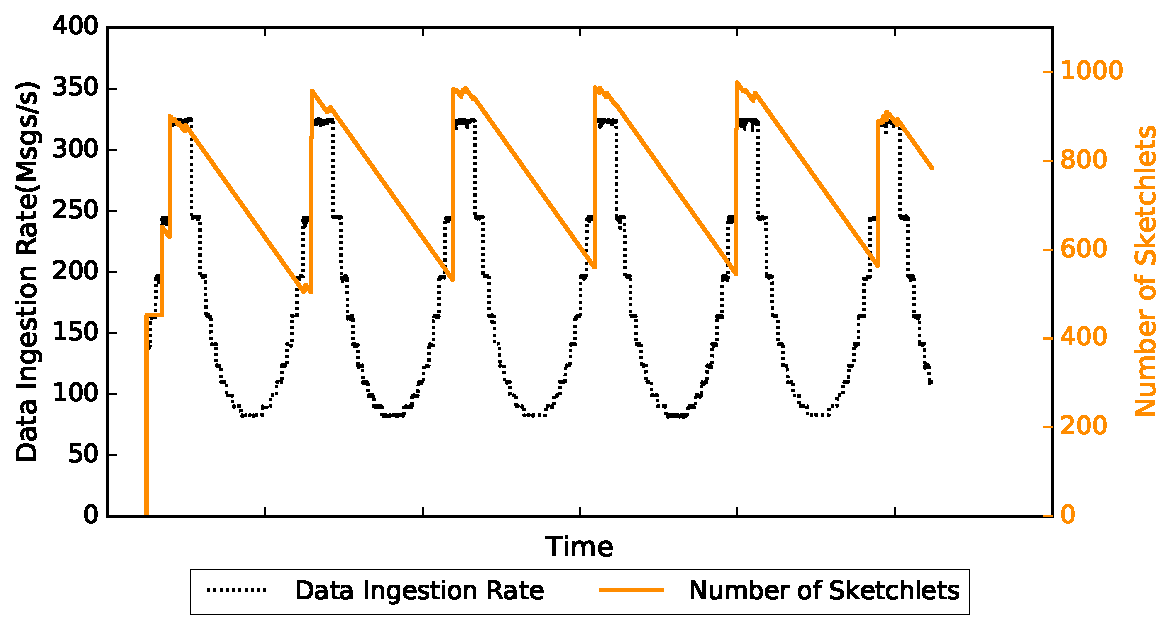
\includegraphics[width=3.5in]{figures/dyn-scaling.pdf}}
    \caption{Variation in the number of sketchlets as the data ingestion rate changes.}
    \label{fig:dyn-scaling}
\end{figure}
We evaluated how \textsc{Synopsis} dynamically scales when the data ingestion rate is varied.
The data ingestion rate was varied over time such that the peak data ingestion rate is less than the highest possible throughput that will create a backlog at \textsc{Synopsis} nodes.
We used the number of sketchlets created in the system to quantify the scaling activities.
If the system scales out, more sketchlets will be created in child nodes after the targeted load migration.
We started with a single \textsc{Synopsis} node and allowed the system to dynamically scale.
As can be observed in Figure~\ref{fig:dyn-scaling}, the number of sketchlets varies with the ingestion rate.
Since we allow aggressive scale-out, it shows rapid scaling activity during high data ingestion rates whereas scaling in takes place gradually with one sub region (hence one sketch) at a time.

\subsection{Analyzing a Snapshot of the Distributed Sketch}
% scale out graph
\begin{figure*}[t!]
    \centerline{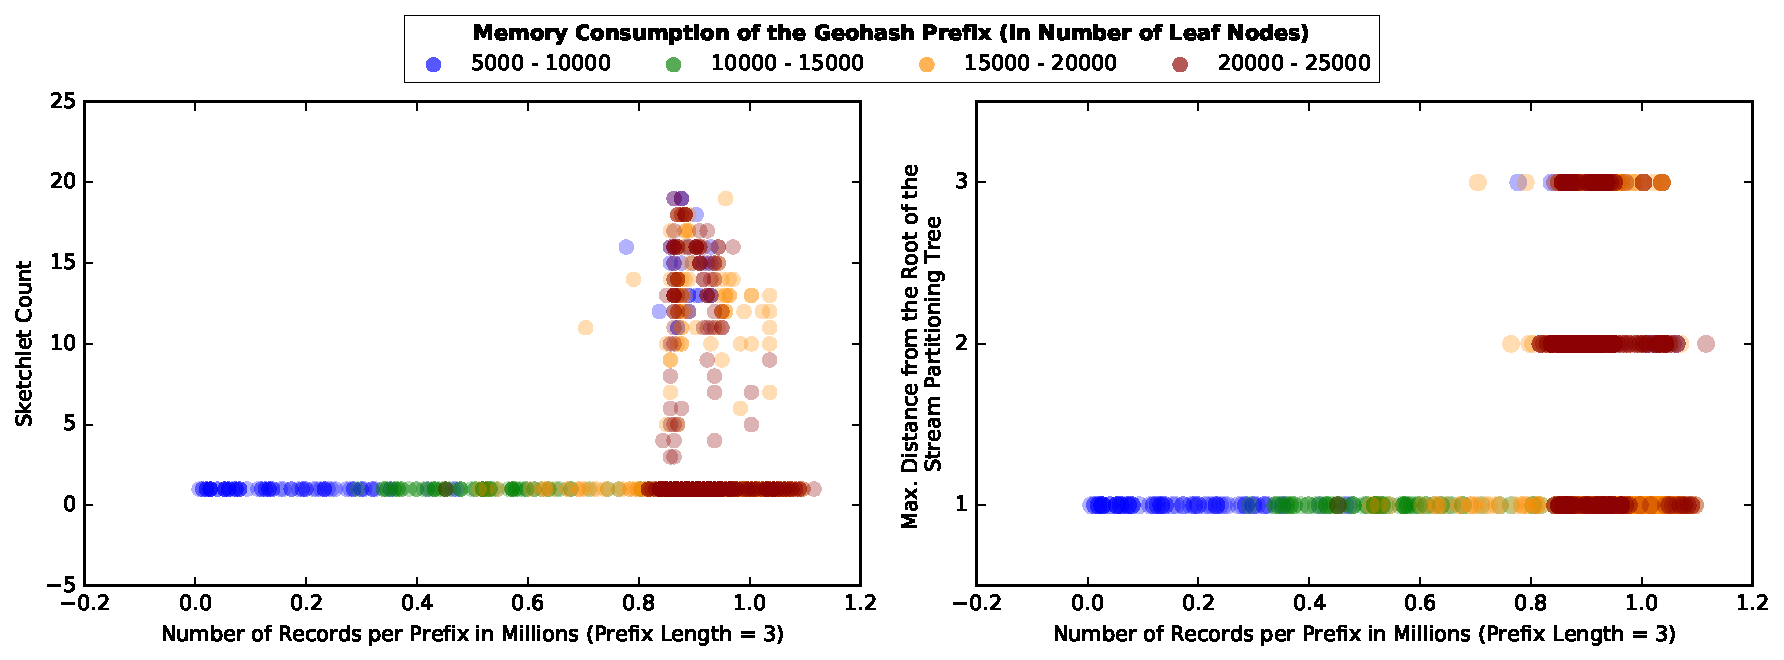
\includegraphics[width=\linewidth]{figures/scaleout_graph_analysis.pdf}}
    \caption{Analysis of a snapshot of the stream processing graph during data ingestion demonstrating the size and distribution of the information corresponding to different prefixes against the observed record count. If the information is dispersed over multiple sketchlets, it is likely to be a prefix with higher number of records and/or a wide range of observed values.}
    \label{fig:scaleout-graph-analysis}
\end{figure*}
%
Figure~\ref{fig:scaleout-graph-analysis} visualizes a snapshot of the stream processing graph in runtime which demonstrates the stream partitioning concepts discussed above. 
This represents the state of the system after consuming the complete NOAA dataset for 2014 and the graph contained 48 sketchlets. 
It shows the distribution and size of the information maintained across \textsc{Synopsis} nodes for each geohash prefix of length 3 against the number of records processed for that particular prefix.
The memory requirement for a particular geohash prefix depends on the number of records as well as the range of the observed values for different features.
The space requirement is measured in terms of the number of leaf nodes in the corresponding sketchlets.
For the majority of the prefixes, the space requirement increases with the number of records processed for a particular prefix.
If the data for a particular prefix is distributed across multiple sketchlets, then it is more likely to be a prefix with a high number of records as shown in the first subplot.
In such cases, some of these sketchlets are created in multiple iterations of scaling out operations from their original nodes which results in a higher distance from the root in the prefix tree. This is depicted in the second sub figure of Figure~\ref{fig:scaleout-graph-analysis}.
A few prefixes with high number of records can be observed with a low memory consumption and are distributed across multiple sketchlets.
Their observations spans across a smaller range, hence requires less memory but they were chosen for scaling out operations due to their high message rates. 

\subsubsection{Distributed Sketch Memory Evaluation}
%
\begin{figure}[b]
    \centerline{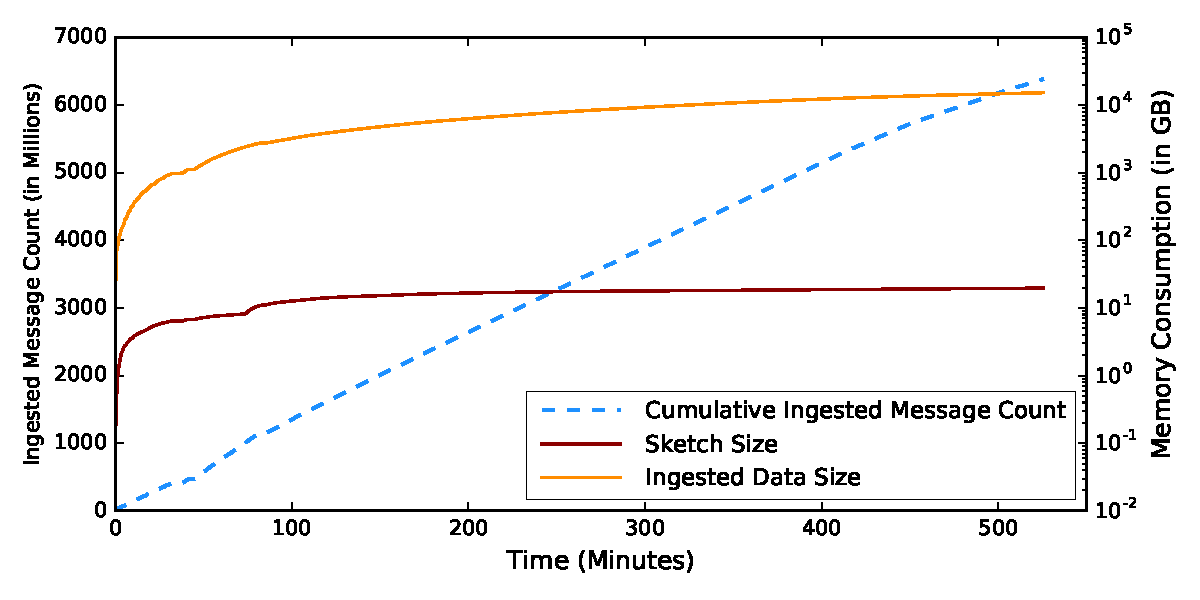
\includegraphics[width=\linewidth]{figures/ing-and-mem-usage.pdf}}
    \caption{Memory usage of the distributed sketch over time against the amount of ingested data. The rate of growth decreases over time due to the compact nature of our underlying sketchlet data structure.}
    \label{fig:dist-sketch-mem-usage}
\end{figure}

We monitored the growth in memory consumption of the entire distributed sketch over time with continuous data ingestion as shown in Figure~\ref{fig:dist-sketch-mem-usage}. This experiment included all 40 of the nodes in our test cluster.  As more data was streamed into the system, the growth rate of the distributed sketch decreased as the sketchlets at each node expanded to include vertices for their particular feature space.  At the end of our monitoring period, the total amount of ingested data was over three orders of magnitudes higher ($\sim 1285$) than the in-memory sketch size, resulting in notable space savings.

\subsection{Query Evaluation Performance}
Figure~\ref{fig:dist-query} demonstrates the end-to-end efficiency of the query evaluations over the distributed sketch.
Cumulative query throughput and latencies were measured with varying numbers of concurrent query \emph{funnels}.
A query \emph{funnel} continuously generates and dispatches random queries at their maximum possible rate to stress test the system and saturate its capacity; for instance, a query could request summary statistics or feature relationships when the temperature is between 20 to 30 degrees, humidity is above 80\%, and the wind is blowing at 16 km/h.
These randomized queries fluctuated in both the ranges of values and spatial scope, resulting in high variability in the number of \textsc{Synopsis} nodes required to resolve the query as well as the depth and breadth of the required graph traversals.

\begin{figure*}
    \centerline{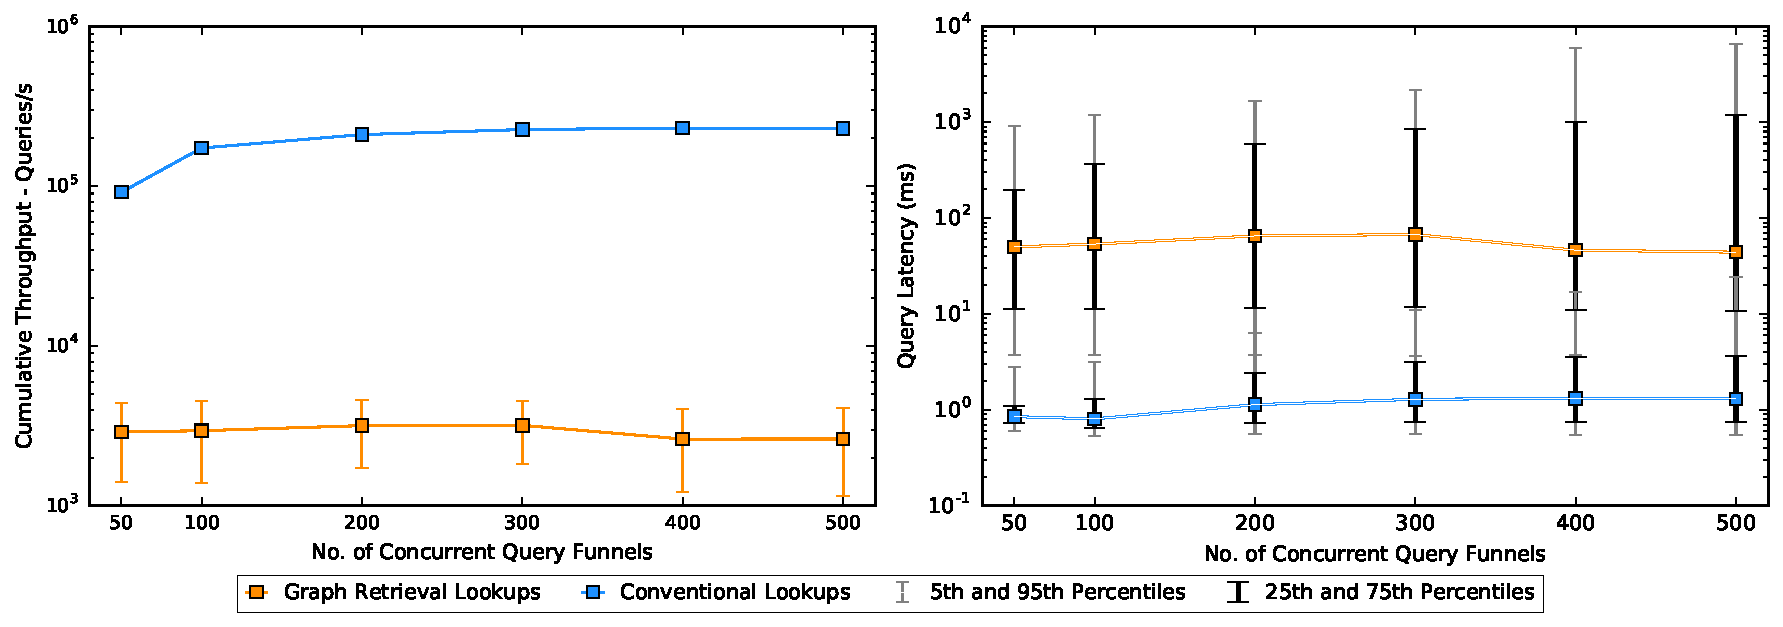
\includegraphics[width=\linewidth]{figures/query_benchmark_both.pdf}}
    \caption{Distributed Query Evaluation Performance. Variation of cumulative throughput and latency against the number of concurrent query funnels in a 40 node \textsc{Synopsis} cluster.}
    \label{fig:dist-query}
\end{figure*}




